%%%%%%%%%%%%%%%%%%%%%%%%%%%%%%%%%%%%%%%%%%%%%%%%%%%%%%%%%%%%%%%%%%%
%                                                                 %
%                            CHAPTER TWO                          %
%                                                                 %
%%%%%%%%%%%%%%%%%%%%%%%%%%%%%%%%%%%%%%%%%%%%%%%%%%%%%%%%%%%%%%%%%%%

\chapter{LITERATURE REVIEW}\label{ch:prevwork}
%\resetfootnote %this command starts footnote numbering with 1 again.

\section{Introduction}

The data versioning landscape produces a variety of different approaches and standards towards change capture.
Science agencies and organizations are only beginning to formally codify and standardize methods to capture and publish lineage information \cite{MatthewS.Mayernik201312-039}.
In comparing their methods, many systems also share the implementation of common versioning operations, suggesting an avenue for fundamental versioning properties.
While Software Versioning Managers (SVM) prefer to adopt the dot-decimal identifier, Digital Object Identifiers (DOI) and other web identifiers contribute methods to connecting more expressive change documents.
Change logs are a feature which commonly appears alongside software projects and provide insight in differences between versions, but they are found very rarely among data sets.
Measuring the space between versions also appears under-explored in previous approaches.

\section{Current Versioning Models} \label{sec:models}

Version models provide a visual theoretical aid in understanding where a data object lies in relation to the rest of a work.
The \gls{arm} group at Pacific Northwest National Laboratory used a model dividing the data into mathematical sets which versioning operations acted upon\cite{6906868}.
Adding files already in the set created a new set which inherited all non-intersecting files and included all the new ones.
The model provided a means to organize and automate the versioning of \gls{arm}'s daily expanding data sets.

The \gls{hcls} Interest Group of the \gls{w3c} recently released a model which resembles the \gls{frbr} model with a three level hierarchy of increasing granularity \cite{Dummontier2016}.
Their model, shown in Figure \ref{HCLSModel}, separates the concept of a data set into three groupings.
\begin{figure}%[b]
	\centering
	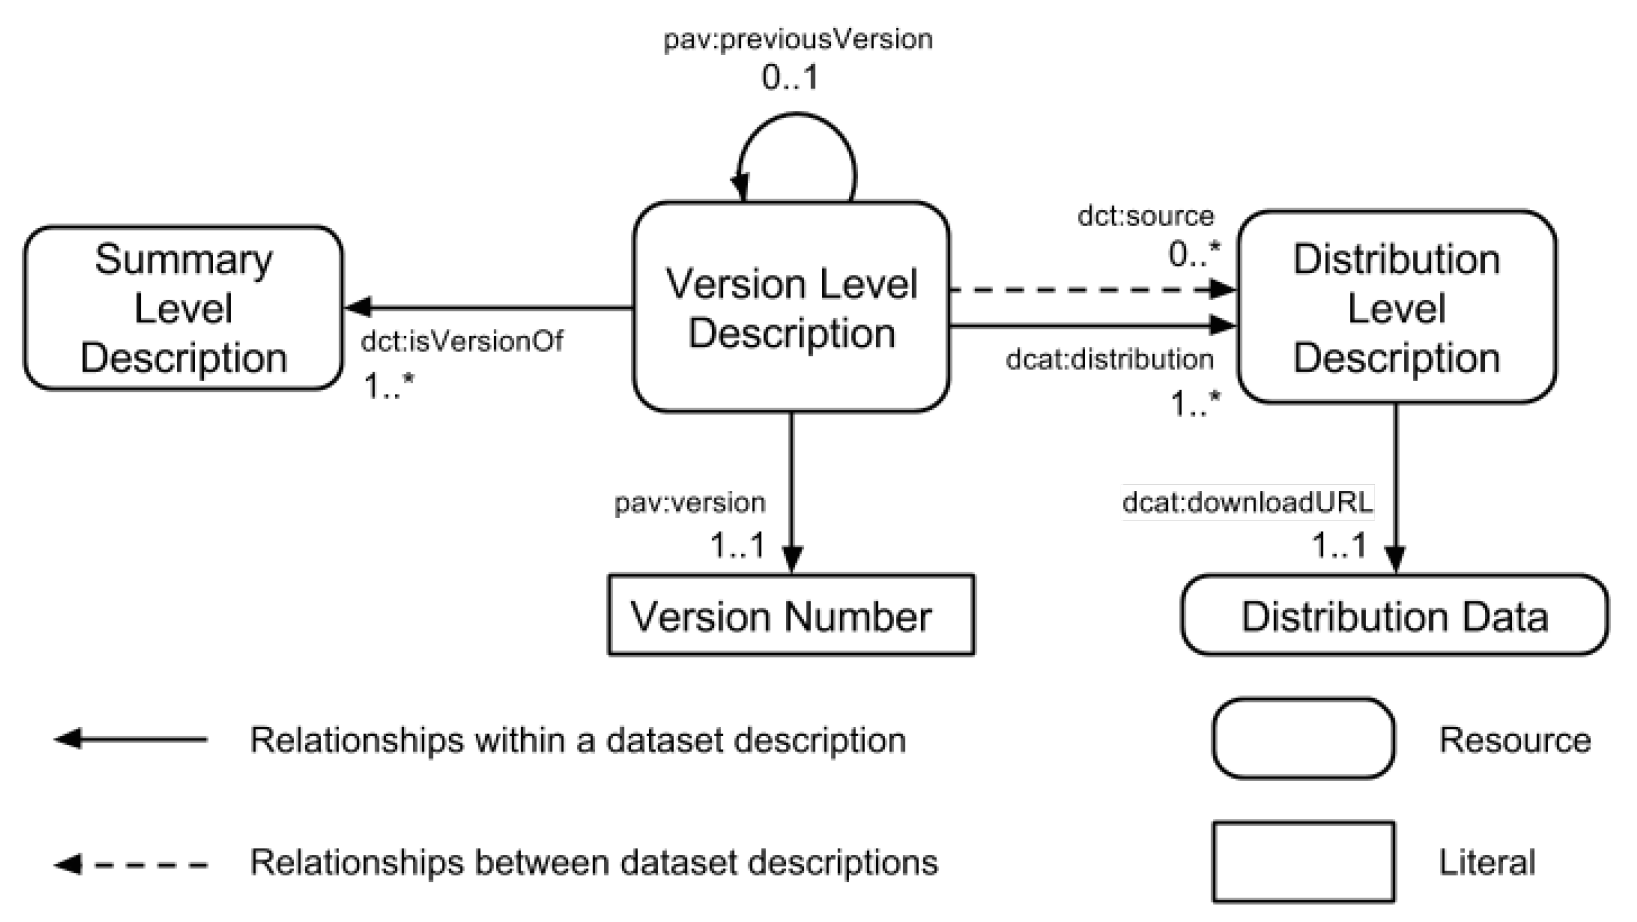
\includegraphics[scale=0.34]{figures/HCLSModel.png}
	\caption[Data model from the W3C's Health Care and Life Sciences Interest Group separating data into three levels: works, versions, and instances.]{Data model from the W3C's Health Care and Life Sciences Interest Group separating data into three levels: works, versions, and instances.  From Dummontier, et al. \cite{Dummontier2016}}
	\label{HCLSModel}
\end{figure}
The highest level summarizes the data as an abstract work, perhaps better described as a topic or title.
The data topic can have multiple versions over time.
The version can then be instantiated into various distributions with different physical formats.
The model---relating summary, version, and distribution---provides a method to implement the formation of \gls{frbr}'s work, expression, and manifestation model on the Web.

From his definition of versions, Barkstrom also outlines a hierarchical version model as seen in Figure \ref{hierarchy}.
\begin{figure}
	\centering
	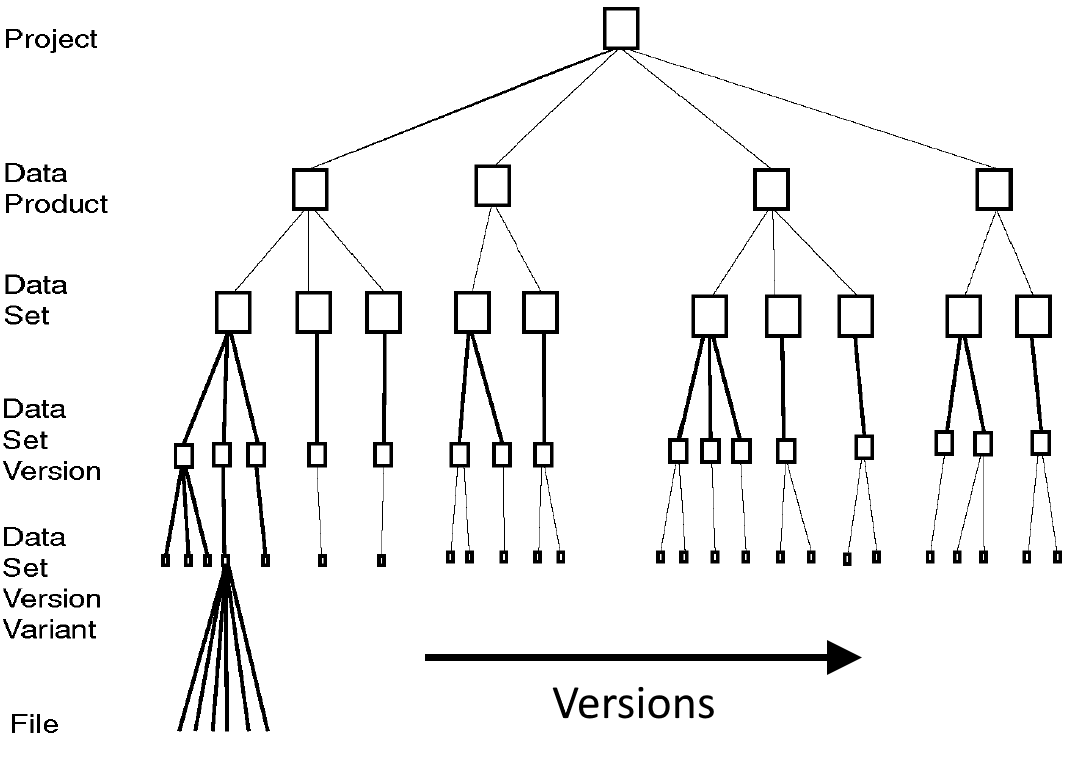
\includegraphics[scale=0.50]{figures/hierarchy.png}
	\caption[Visual representation of grouping hierarchy.]{Visual representation of grouping hierarchy.  Each row of the hierarchy defines a level of granularity where differences can separate ``homogenous groupings" of data.  From \cite{Barkstrom2003}}
	\label{hierarchy}
\end{figure}
The model features more intermediary levels than the \gls{hcls}'s model by introducing data products and data sets as ``homogeneous groupings" where differences can be introduced \cite{barkstrom2014earth}.
Each edge in the tree signifies a difference with other objects at the same depth, but the model does not provide a mechanism to explain the difference.
The difference in the number of tiers employed in the \gls{hcls} and Barkstrom models also indicates that different applications will have varying expectations of granularity to their versioning models.
Granularity is important because it defines the detail with which versioning activities will be executed.
A general solution will likely need to be tiered and recursive in structure to accommodate different levels of specificity.

\section{Documenting Versions} \label{sec:changelog}

When workflow activities generate new \glspl{version} of a data object, connective tissue becomes necessary to bind the \glspl{version}.
\Glspl{log}, artifacts resulting from the versioning process, play a major role filling in gaps between versions.
\Glspl{log} document changes and explain, in human language, motivations behind the differences \cite{uel1037}.
Introducing \gls{log} information into \gls{linked} follows logically from the drive to improve transparency of characteristics connecting data sets, a \gls{linked} principle.
Very little evidence exists suggesting that \gls{log} data is being captured by \gls{linked} practices.
The provenance ontologies covered in Section \ref{sec:provmod} contain terms which are too broad to express changes at the same level of detail as \glspl{log}.
\gls{nasa} Earth Science's treatment of versions has been found to vary depending on a data community's traditions, meaning that if an ontology to express change data existed, the ontology may not be applicable to every community due to opposing traditions \cite{barkstrom2014earth}.
A review of data versioning in biology also identifies the lack of a standardized versioning format suggesting the lack of an accompanying standardized method to consume versioning data \cite{Tagger2005}.
While some data sets will contain a \gls{log}, software projects have normalized their use in version release documentation \cite{German03automatingthe}.
The popular \gls{svm} Git provides methods to attach messages to commits, but the messages are in plain-text rather than a \gls{linked} compatible format \cite{Chacon:2009:PG:1618548}.
As a result, software projects provide a basis for understanding the value of \glspl{log} to data sets with multiple \glspl{version}.
Drawing trends from \gls{log}s is limited by only appearing in human readable text.
Wider adoption among data sets may be possible by making change texts machine readable.

The following studies demonstrate the value that can be unlocked by studying the behaviors and data stored within software \glspl{log}.
\Glspl{log} play an important communication role in open-source projects, allowing new developers to trace implementation decisions made through the life-cycle of a project.
In one project, researchers explicitly linked \gls{log} entries to documented bug reports, showing how bugs of different priorities were addressed \cite{Chen:2004:OCL:990374.990391}.
The links give insight into motivations behind particular implementation decisions.
\Glspl{log} linked with \gls{version} releases also provide feedback to the user community that issues have been addressed, in addition to ensuring that improvements drive modifications to the code base.
The rate of \gls{log} release has been shown to be a good indicator for the general health and activity within a software project \cite{German03automatingthe}.
The poor health of a project can negatively impact adjacent systems.
A project mined change histories to determine dependency patterns in source code changes which would cause a cascade of follow-up bugs in other projects \cite{6132954}.
The research is pertinent to systems which rely on multiple projects to function, but also functions very similar to inter-operable data systems like those created by \gls{linked}.
The change history mining project diverges from previous approaches by looking primarily at the presence of differences between the source code instead of the natural language text in accompanying logs.

\section{Provenance Representation} \label{sec:provmod}

\Gls{linked} is a collection of methods standards which improve data set interoperability by using technology to expose the characteristics and connections between collections of data on the Web of Data \cite{ld}.
Provenance ontologies form a major section of \gls{linked} approaches to data versioning.
The coverage stems from the close relation between provenance and differentiating versions.
The Proof Markup Language, one of the first semantic models to capture provenance information, expressed lineage relationships using inference reasoning through traceable graphs \cite{daSilva2006381}.
The technique provides a powerful way to express and imply sequences of relationships between different versions and characterize the manner of their relation.

\subsection{Open Provenance Model}

\gls{opm} was the product of a series of provenance challenges held at International Provenance and Annotation Workshops after participants began realizing and reaching consensus on the formulation and content of provenence information necessary to establish system interoperability \cite{moreau2008open}.
In a project, the model has been applied to sensor networks, automating and unifying their provenance capture even as they grow \cite{5478496}.
To aid \gls{opm}'s adoption, the framework Karma2 integrates provenance capture into scientific workflows and provides a more abstract view of their data collection activities \cite{simmhan2010karma2}.
The property \textit{opm:WasDerivedFrom} constitutes a core concept in the model and marks the reliance of one object's existence on another object.
For a large part, the relation encompasses the engagement which provenance models view versions, without further need to explore the derivation's content.

\subsection{PROV-O}\label{sec:prov}

\gls{prov}, a \gls{w3c} Recommendation, delineates a method to express data provenance in a more compact form as seen in Figure \ref{PROVO} \cite{Gil2013a} \cite{Groth2013}.
\begin{figure}
	\centering
	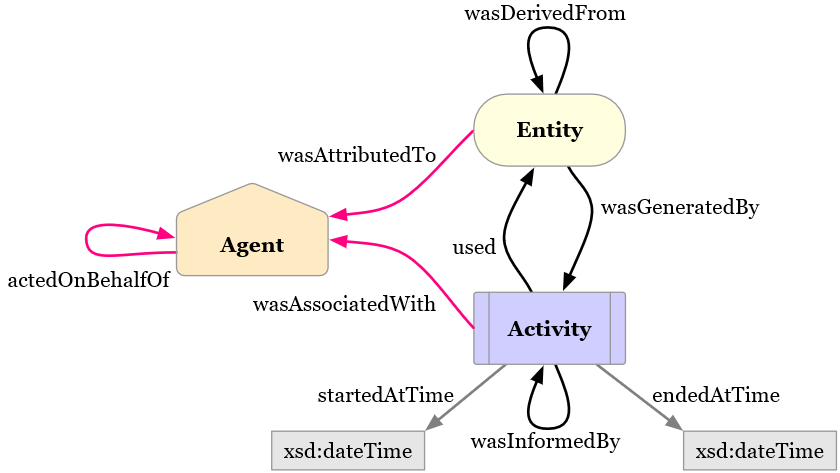
\includegraphics[scale=0.5]{figures/ProvO.png}
	\caption[Diagram of the PROV Ontology.]{The PROV Ontology is divided into three main objects: Entity, Agent, and Activity.  An Activity is an action or process which produces Entities which is associated with an Agent.  Agents are usually individuals responsible for creating Entities.  The high level ontology can capture complex provenance relationships to ensure traceability of data production.  Figure 1 from \cite{Lebo2013}}
	\label{PROVO}
\end{figure}
The recommendation uses a conceptual model relating activities, agents, and entities to describe data production lineage, the list of data ancestors leading to a data object \cite{Moreau2013c} \cite{Nies2013} \cite{Nies2013a}.
Intended as a high-level abstraction, \gls{prov} takes an activity-oriented approach to provenance modeling.
Every data entity results from the actions of some activity \cite{Gil2013}.
The conceptual model's expression occurs through the \gls{prov} Ontology (PROV-O), which is conveyed through various resource description languages \cite{Hua2013} \cite{Klyne2013}.
The ontology is further formalized into a functional notation for easier human consumption \cite{Moreau2013b} \cite{Cheney2013a}.
One particular strength that has contributed to the adoption of \gls{prov} is its ability to link into other ontologies, making it easier for existing semantically enriched data sets to adopt \gls{prov} \cite{Miles2013} \cite{Moreau2013}.

\gls{prov} has provided a major contribution in maintaining the quality and traceability of data sets and reporting in the \gls{nca} published by the U.S. Global Change Research Program \cite{Ma2014191}.
The inclusion into the \gls{nca} signifies that there is an increased likelihood of adoption through other scientific fields as a result of this reporting.
The Global Change Information System, which houses the data used to generate the \gls{nca} and maintained by the U.S. Global Change Research Program, uses \gls{prov} to meticulously track the generation of its artifacts and results as they are used in the assessment report \cite{Tilmes2012}.
Usage means that not only does the data have a traceable lineage to verify quality, but the content of documents can have the same verifiability \cite{Ma2014}.

Komadu, a framework developed to alleviate workflow integration, utilizes PROV to improve upon its predecessor, Karma, by no longer utilizing global context identifiers that were not necessarily shared throughout the workflow. \cite{Suriarachchi_2015}.
The framework and the adoption of \gls{prov} in high profile scientific applications means versioning applications can be overlayed onto a \gls{provenance} skeleton once a versioning ontology has been created.

The \gls{prov} Ontology provides three different concepts that begin to encapsulate the provenance relationship between data versions.
It defines a \textit{prov:Generation} as ``the completion of production of a new entity by an activity," \cite{Lebo2013}.
The definition means that the generation, which corresponds to adding an object to a version, must result from a \textit{prov:Activity}.
\textit{Prov:Invalidation}, defined as the ``start of the destruction, cessation, or expiry of an existing entity by an activity," makes a similar connection between activities and entities \cite{Lebo2013}.
A third concept, \textit{prov:Derivation}, relates two entities, and the ontology defines it as, ``a transformation of an entity into another, an update of an entity resulting in a new one, or the construction of a new entity based on a preexisting entity. " \cite{Lebo2013}.
PROV also has a property called \textit{prov:isDerivedFrom} which conveys the same definition as a \textit{prov:Derivation}.
Using the property and concept together forms a qualified property which can be instantiated and further annotated.

\subsection{Provenance, Authorship, and Versioning Ontology}

The \gls{pav} Ontology is, ``a lightwei\-ght vocabulary, for capturing ``just enough" descriptions essential for web resources representing digitized knowledge" \cite{Ciccarese2013}.
It provides a means to track versioning information through linked data by introducing \textit{pav:version} to cite versions and \textit{pav:previousVersion} to link them together in order \cite{Ciccarese2013}.
The authors of \gls{pav} created the new property to expand on the Dublin Core concept \textit{dc:isVersionOf} which is used when, ``Changes in version imply substantive changes in content rather than differences in format" \cite{DCMI2012}.
\gls{pav} supports the idea that a new concept becomes necessary to cover cases where new \glspl{version} do not have to be substantive but can still be alternate editions of the original object.
While it documents related versions well, \gls{pav} does not dive deeper in explaining the circumstances behind version differences.

\subsection{Schema.org}

\sloppy
The Schema.org structured data schema is not a provenance ontology but provides a means to supply searchable web pages with standardized micro-data.
The schema has a collection of concepts which could be applied to versioning.
The \textit{schema:UpdateAction} is defined as, ``the act of managing by changing/editing the state of the object," which encompasses the same responsibilities expected of versioning systems \cite{Schema}.
The terms \textit{schema:AddAction}, \textit{schema:DeleteAction}, and \textit{schema:ReplaceAction} subclass the \textit{schema:UpdateAction}.
These classes model actions which further cement parallels between versioning and \textit{schema:UpdateAction}.

\fussy
Schema.org defines a \textit{schema:ReplaceAction} as, ``the act of editing a recipient by replacing an old object with a new object" \cite{SchemaRep}.
The concept has two properties, \textit{schema:replacee} and \textit{schema:replacer} which indicates that a new object replaces an old one.
Schema.org models the interaction by placing the replacement action at the relation's center.
In comparison, the \textit{schema:AddAction} is defined as, ``the act of editing by adding an object to a collection" \cite{SchemaAdd}.
The action only involves the object and the new state of the collection, not involving any of the collection's prior lineage.
Schema.org defines the \textit{schema:DeleteAction} as, "the act of editing a recipient by removing one of its objects," \cite{SchemaRem}.
The concept aligns well with other versioning systems, although deletion may be a strong assertion.
The deletion would be inappropriate for use in cases where data is archived but no longer used, for example or when data becomes deprecated.

Provenance models are a necessary step towards the development of versioning models.
Going back to the working definition of a version and the discussion from Barkstrom, \glspl{version} are produced from changes to \gls{provenance}, and without the ability to clearly trace \gls{provenance}, \glspl{version} cannot be clearly organized.
A number of \gls{linked} \gls{provenance} models include versioning concepts such as \gls{opm}, \gls{prov}, and \gls{pav}.
Each model approaches versioning differently, ranging from very broad to very narrow definitions of a \gls{version}.
None of the models approach capturing the differences between \glspl{version} which is appropriate since the differences do not explain the processes used to create a digital object \cite{moreau2008open}.
Versioning, in contrast, documents the results of using a different process.

\section{Version Systems} \label{sec:system}

Versioning systems take many different forms from Clotho, an application conducting versioning at the block level, to Champagne, a framework to propagate change data across multiple information systems \cite{Flouris04clotho:transparent} \cite{Systems02champagne:data}.
Each approach has a unique set of challenges to overcome.
Closer to the data collection, version systems must be flexible and responsive to adapt to changing environments, but as the socio-technical distance of a repository increases away from the collection site, more formal methods are required to unify repositories \cite{Baker2009}.
Different approaches are also necessary to account for the needs of different domains.
Versioning an XML text-file will need to account for serial file input and output as well as structured markup \cite{Chien:2000:VMX:646544.696357}.
Many applications have adopted a tree-like structure which is further propagated by software versioning managers (SVM) \cite{Stuckenholz:2005:CEV:1039174.1039197}.
The advantage comes from using well established graph theory methods, and applying the methods to an object's complex relationships in complex environments \cite{Dijkstra1994}.
The growing population of web documents, however, presents a new smörgåsbord of complicated data which will need scalable solutions \cite{Berberich:2007:TMT:1277741.1277831}.

\subsection{Library Sciences}

While many of the modern systems requiring versioning managers store digital products, libraries have been tackling similar issues for a much longer time.
Libraries curate multiple editions of the same work, sometimes with significant revisions \cite{Wiil:2000:RDH:338407.338517}.
In many ways, versioned objects resemble multi-edition books or documents.
Digital librarians have faced many challenges when searching for a persistent identifier due to evolving web technologies.
Early citations referred to on-line documents using stagnant \gls{url}, but this frequently lead to a condition known as link rot where moving the document would invalidate the URL \cite{Lyons2005}.
Locators required a system to manage changes of old identifiers to new locations when people attempted to utilize references from print.
The need eventually led to the development of \glspl{purl}, which also suffered from link rot, and this eventually led to the distributed \gls{doi} system used to track documents today \cite{Duerr2011}.
The \gls{purl} used a centralized system that would translate dead links and redirect to a document's latest location.
The system would still need to be manually updated, meaning links would rot if a document was lost or overlooked.
\Glspl{doi} rely on a network of managing agencies to collect and host submitted documents.
In the specialized Handle system, the network has member agencies internally assign an unique name and concatenate it to the end of their host name.
In Figure \ref{table:Duerr}, \glspl{doi} represent the most suitable identifier used for citation in scholarly literature \cite{Duerr2011}.
\begin{figure}
	\centering
	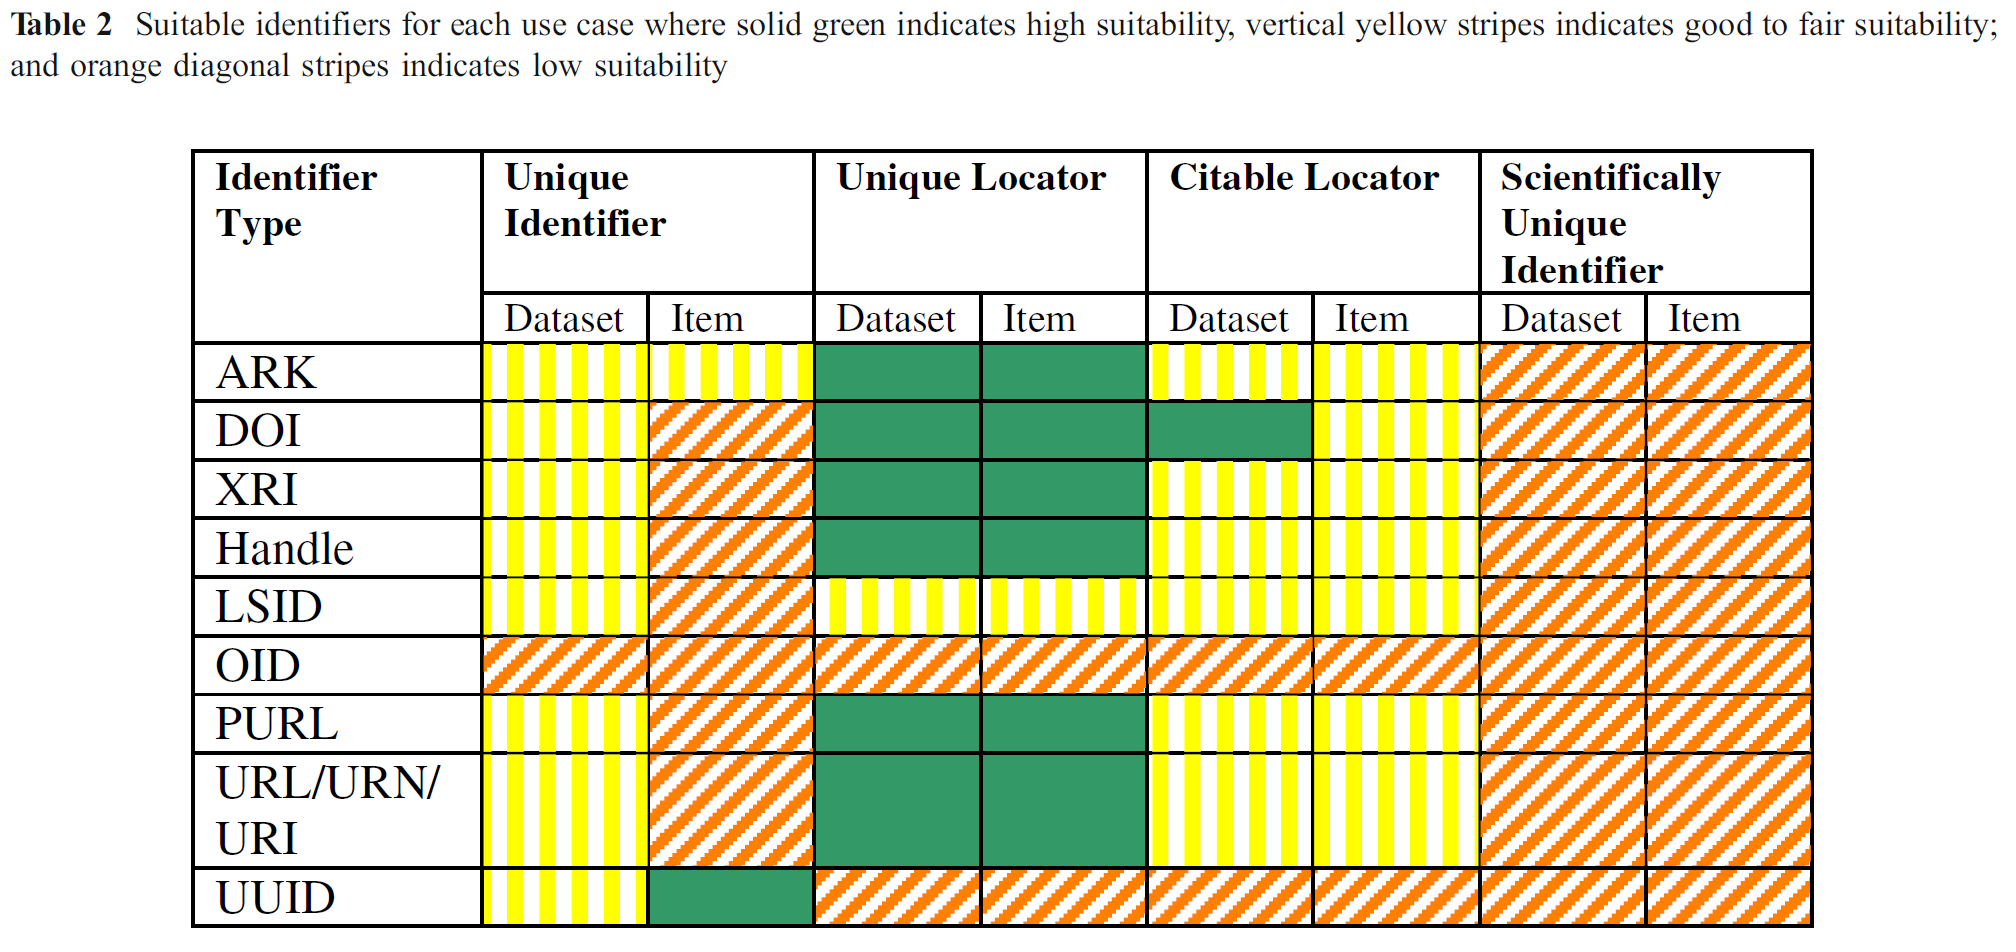
\includegraphics[scale=0.28]{figures/DigitalIdentifierTable.png}
	\caption[Table of predominant identifiers used in science.]{Table of predominant identifiers used in science.  From Duerr, et al. \cite{Duerr2011}}
	\label{table:Duerr}
\end{figure}
The \gls{doi} network provides a robust system to track documents, but when tracking data, it faces difficulty following the rate of change with more volatile data sets.
Under current definitions, distribution organizations assign different \glspl{doi} to separate editions of a document.
Documents often do not need new identifiers since they change very rarely as a result of the publication process.
Data set production and distribution cycles move more quickly and react more sensitively to small content changes, including when data collection continues on after initial publication.
Data set behavior becomes entirely too slow as data providers begin allowing users to dynamically generate data products from existing data according to their needs \cite{Barkstrom2003a}.
Some agencies have begun assigning versioned \glspl{doi}, but this has not become common practice.
Other groups do not assign a new \gls{doi}, but reference the latest release of the document or object \cite{Ands2017}.

As digital methods have evolved, so have digital libraries.
The documents that digital libraries store are no longer constrained by physical organization \cite{Barkstrom_digitallibrary}.
A book can physically be randomly stored for efficient retrieval, but the digital copy may reside in multiple locations depending on dynamic filters or search queries.
The Mellon Fedora Project developed a standardized edition control structure to unify disparate digital library stores \cite{Payette2002}.
The regularizing edition tracking methods significantly improved the response time and relevancy of the library services.

\subsection{Software Versioning}

Software versions form the most visible displays of versioning often experienced by researchers.
Version managers provide tools to archive and restore code through the development lifecycle.
The \gls{rcs}, developed in originally in 1985, documents one of the earliest uses of the dot-decimal identifier \cite{tichy1985rcs}.
This identifier uses a sequence of whole numbers concatenated by decimals.
The system possessed many features of modern \glspl{svm} such as branches, a separate copy of the code for developing changes safely, which were identified by extending the dot-decimal identifier as seen in Figure \ref{RCSTree}.
\begin{figure}
	\centering
	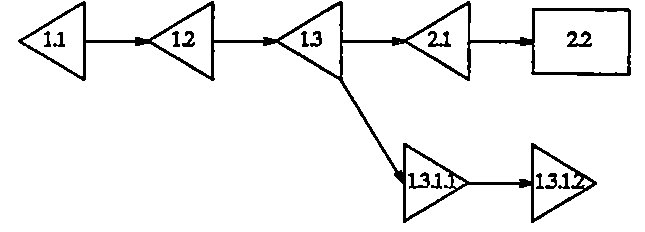
\includegraphics[scale=0.75]{figures/RCSCommitTree.png}
	\caption[Commit history of an object in RCS with changes in the main line stored as back deltas and side branches stored as forward deltas.]{Commit history of an object in RCS with changes in the main line stored as back deltas and side branches stored as forward deltas.  Figure 5 in \cite{tichy1985rcs}}
	\label{RCSTree}
\end{figure}
Not long after, the \gls{cvs} gained popularity with methods allowing multiple users to concurrently develop code to a central repository \cite{cederqvist2002version}.
The most popular modern \gls{svm} is Git which also allows concurrent development but enables distributed repositories \cite{Chacon:2009:PG:1618548}.
Each developer contributing to a project is considered by the system to possess the master copy of that project.
The users collaborate by requesting and pulling other developer's master copies into their project.
In previous \glspl{svm}, only the differences between software files were stored, but Git stores the entirety of each file version.
Figure \ref{GITFile} demonstrates an example of how Git employs storage space for multiple versions \cite{Chacon:2009:PG:1618548}.
\begin{figure}
	\centering
	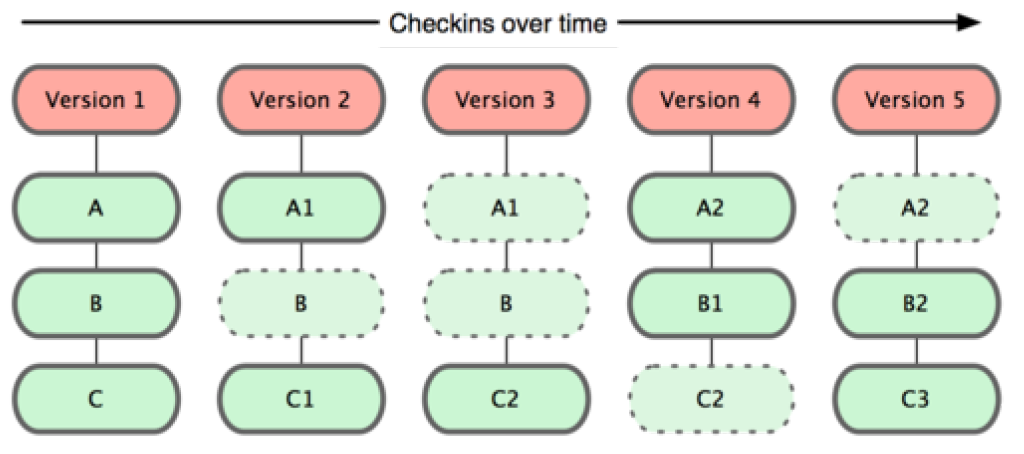
\includegraphics[scale=0.50]{figures/GITFiles.png}
	\caption[Git stores changes in the repository as snapshots of individual files.]{Git stores changes in the repository as snapshots of individual files. Figure 1.5 from \cite{Chacon:2009:PG:1618548}}
	\label{GITFile}
\end{figure}
Only a pointer is stored in subsequent versions for unchanged files, saving space.
Fischer, et al., demonstrate the importance of software version systems by integrating the manager with a bug tracking system to indicate the bugs a version release addresses \cite{Fischer2003}.

\subsection{Database Versioning}

The need for data versioning methods grew alongside the growing popularity and power of relational databases.
Klahold, et al., introduced using abstract versioning environments in 1986 to separate the temporal features and organize the data into related groupings \cite{Klahold:1986:GMV:645913.671314}.
Research in the versioning area focused primarily on the database schema.
The results were temporal databases where schemas included time and dated transactions modifying the schema \cite{roddick1996model}.
Temporal databases allowed old queries to be executed on updated schemas, improving the reproducibility of results.
Capturing periodic snapshots or copies becomes unfeasible with increasingly large centralized database systems.
Data collection continues to migrate towards massive data warehouses which store and serve a wide variety of data \cite{Vassiliadis1999}.
Proell and Rauber have investigated tracking data queries instead of the database as a more scalable solution to reproduce data \cite{proellBigData}.
The queries can then be used as publication citations to provide scalable, reproducible references to older data \cite{Proell2013} \cite{DBLP:conf/data/2013}.

\subsection{Grid Versioning} \label{sec:grid}

The grid provides a sensitive environment for versioning where there are many users and data movement across the grid should be avoided.
The CERN grid for the Compact Muon Solenoid experiment carefully developed processes which allow references by multiple users to the same file without copying that file across the grid \cite{Holtman:687353}.
Versions lock and release to permit parallel processing while still archiving additions and modifications to the data.
Grid versioning applications also begins to highlight the difference in versioning usage patterns between users and producers \cite{Branco2008}.
Deeper exploration into the \gls{atlas} system documentation did not reveal specific use cases explaining the differences.
The grid also provides users with the ability to begin dynamically defining data sets to their needs by aggregating results from across the network \cite{Barkstrom2003a}.
The process would create new data sets without prior existing change documentation and fueled a demand for responsive frameworks which could track the discordant data collection conditions assimilated by the system \cite{Kovse2003VGridAVS}.

\subsection{Ontology Versioning}

Ontologies play a major role in defining domains, especially in the biological and medical fields where terms and definitions can change rapidly across highly variable organisms \cite{Ochs:2015:SVS:2826733.2826866}.
As a result, the ontologies require consistent methods to capture and model changes to evolving terms.
Tools aid in the process by detecting differences between ontologies \cite{Hartung201315}.
Klein and Fensel have found that when the changes are discovered, both forward and backward compatibility must be established for clear ontology versioning \cite{Klein01ontologyversioning}.
Not only must the path from an old term to a new one be clear, but a method for new terms to interact with old data must also exist.
They additionally identified three levels at which ontologies can differ: the domain, the conceptualization, and the specification.
Hauptmann et al., define a method to version ontologies natively within a triple store using linked data \cite{HauptmannEtAl:LDQ2015} \cite{LDQ2015}.
The method heavily relies on the context of stored data.

\subsection{Evaluation}

Versioning systems cover a wide variety of different application environments, and each uses terminology to define versions in the context of their particular domain.
Application based systems such as software and grid versioning focus primarily on identifying large, medium, and small differences between versions.
The size approach suffers many drawbacks as a result of variety in versioning environments.
Small changes logged in Clotho would barely register in massive systems operating on the grid.
The requirements to differentiate changes is not universal across versioning systems.
Other than software version managers, the systems do not incorporate methods to include change logs.
They use the existence of an alternate version as sufficient explanation for what has changed.
Bose, Frew, and Tagger all recognize the need in versioning for a standardized representation, but each domain defines change according to the needs of their application \cite{Bose:2005:LRS:1057977.1057978} \cite{Tagger2005}.
In isolation, the systems to not recognize the commonality in utilizing similar operations to conduct versioning activities.

\section{Data Versioning Operations}

Among all the systems surveyed in Section \ref{sec:system}, every one employed some form of the operations add, delete, and modify.
Literature surveys often expect versioning systems to interact with data uniformly because they are asked to perform the same functions \cite{Tagger2005}.
Different data sets, however, may utilize each of the three core operations at different rates \cite{rohtua}.
The differences help to characterize the data set in ways such as a growing set with many additions, a stable collection featuring occasional corrections, or a wildly volatile data set consisting of often deleted and replaced data files.
Understanding these would give insight into the maturity and health of a data set.

While data addition and modification remain fairly uncontroversial, there is a mild division between practical and theoretical approaches to data deletion \cite{Flouris04clotho:transparent}.
A removed object provides evidence of an erroneous activity's results or intermediary steps leading to a final product.
As a result, version management should maintain and track invalidated data instead of deleting it.
The software versioning manager Git uses a method of compressing older data to conserve space without deleting the data \cite{Chacon:2009:PG:1618548}.
Available storage space places pragmatic constraints on the number of projects which can adopt snapshotting practices.
In applications which cannot recover erroneous data nor use it as documentation artifacts, like corrupted surveillance images.
Some high energy physics experiments cannot re-collect observational data due to cost, and as a result, they cannot replace or re-process poor quality data \cite{Cavanaugh2002}.
While the distinction between `deletion' and `invalidations' remains largely semantic, the terms' use in this document reflects an understanding of the different constraints and requirements placed on versioning systems.
As a result, invalidation is adopted as a broad, general term to also encompass data deletions.

A handful of other operations exist among version managers, but they do not prove ubiquitous across most applications.
Software versioning tools like \gls{rcs} commonly feature branching and merging functions to create a versioning line separate from the stable master branch \cite{tichy1985rcs}.
Branching mostly provides an organizational role in development by allowing developers to experiment without contaminating a stable software release.
Figure \ref{GITTree} models a branching operation, showing versions C3 and C5 in branch iss53 before being merged back into the production line as C6.
Branching allows for more orderly management of versions, but does not conduct versioning itself.
Other activities provide functional operations such as locking and unlocking files from edits to prevent race conditions in branch mergers.
Locks does not introduce any new relationships but allows the tool to operate more smoothly.
Many version control tools, likewise, include functions to display the versioning tree, but this is also an ease-of-use function \cite{Dijkstra1994}.

\begin{figure}
	\centering
	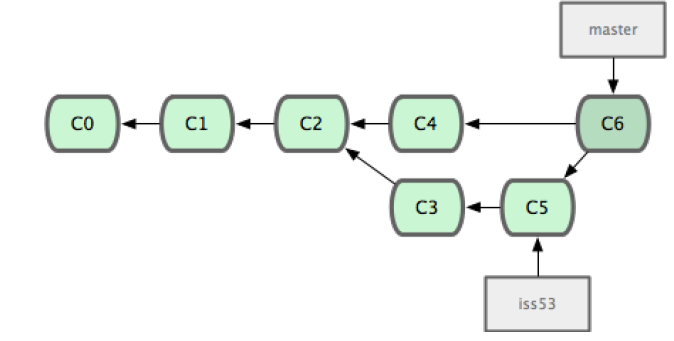
\includegraphics[scale=0.75]{figures/GITCommitTree.png}
	\caption[Example of a commit history with branching stored in Git.]{Example of a commit history with branching stored in Git.  Figure 3.17 from \cite{Chacon:2009:PG:1618548}}
	\label{GITTree}
\end{figure}

\subsection{Types of Change}

Another commonality across many versioning systems is differentiating between major, minor, and revision changes.
Definitions for what constitutes each category differs across applications, but the desire to do so often stems from the tradition of 3-number dot-decimal identifiers.
Barkstrom uses the ability to scientifically distinguish between two data sets as a criteria for major divisions among groupings \cite{Barkstrom2003}.
At lower levels, he notes that science teams can no longer discern scientific differences between data sets.
They observe that, instead, changes to format and structure contribute significant alterations without changing any values withing the data.
As a result, these technical changes form a second boundary to meaningfully separate minor version groupings.
Finally, the explicit values may need occasional revisions to correct lexical errors such as spelling or formatting.
Data producers will often use qualitative measures to determine the type of change occurring between versions.
Versioning system users wish to achieve insight into the type of change that occurs between versions.

The exact category that a particular change falls into can be controversial.
The decision to provide concentration units from parts per million to milligrams per milliliter poses a Technical change for a data producer.
However, for a data consumer, the alteration may be viewed as a Scientific change as it invalidates the methods they had previously used.
The conflict in view illustrates the data consumer-producer dynamic.
In general, data producers control the versioning methods, but data consumers determine a change's impact through use.
Producers tend to use versioning systems to ensure data quality of service through audits and recovery tools \cite{Cavanaugh2002}.
Meanwhile, a consumer will analyze the historical changes and determine the impact this may have on their data use.
As a result, this means that data versioning systems must communicate a dynamic view of the changes in a system contextualized by the user of that data.

Version managers often disagree at the point many technical changes sufficiently modifies a data set that it comprises a scientific change.
As determining changes in science requires expert understanding over a domain, different measures should be explored to address the distinction.

\section{Identifiers}\label{sec:identifier}

The most widely identifier scheme associated with versioning is the dot-decimal identifier \cite{Stuckenholz:2005:CEV:1039174.1039197}.
Whenever, a new version is made, it receives an identifier with one of the numbers incremented as seen in Figure \ref{RCSTree}.
Such a procedure fails to communicate the extent of a change because, regardless of the amount, the identifier will increment only one number.
Changes to the left-most number often signify a more important change.
Many software applications use the 3-number Major.minor.revision format in labeling software releases.
Numbering the version this way, however, does allow computers and readers to quickly parse the version name and discern that a change has occurred, but not much value exists beyond that \cite{Dijkstra1994}.
Most importantly, it groups together changes from the lower spectrum of minor or major change with those in the upper, more impactful, changes.
Obtaining a clear characterization of a version change is difficult without a longer series of numbers.
In addition, version numbers capture the overall change of a data set, but users may not interact with collections that way, only caring about parts of the data or certain kinds of change.
There is also little standardization or formal requirements in naming methods.
Ubuntu utilizes a dot-decimal version labeling scheme where the two number identifier corresponds to the year-month values of the release \cite{Ubuntu}.
A common method used to address the distinction between versions is a human-readable change log, further discussed in Section \ref{sec:changelog}.

The discourse on \glspl{doi} highlights the importance of understanding the limitations of particular identifier schemes.
With respect to Figure \ref{table:Duerr}, no identification scheme fits the description of a scientific identifier.
Duerr, et al., define a use case to make the argument that scientifically unique identifiers are necessary, ``to be able to tell that two data instances contain the same information even if the formats are different" \cite{Duerr2011}.
A possibility to consider is that identifiers may require incorporation into a data model to discern between scientific differences.
An identifier works well in revealing the characteristics of an individual object, but it should not be expected to explain its relationship with other objects.
A data model provides better insight into the different roles objects play in a relationship.
DOIs also provide a new means to identify versions using \glspl{uri} which can be dereferenced to provide change information or the data depending on the context.

Using identifiers to convey extended versioning information becomes more difficult with the adoption of distributed version managers like Git \cite{cederqvist2002version}.
Each participant in the federated repository is the master of their personal copy of the code.
Upon completion of their distribution's part, they may request that it be pulled into another participant's distribution.
While each developer's individual repository can follow a linear identifier scheme, the identifiers would not work as the overall project bounces around different primary repositories with mismatching sequential identifiers.
The dot-decimal identifier scheme could be made to work in such an environment by severely limiting the distributed manager's utilized features.
Figure \ref{fig:federated} illustrates a workflow which utilizes distributed repositories to manage very active public software projects.
Each lieutenant developer manages a section of the overall code, and they dampen the number of requests made to the dictator by collecting changes and submitting them over longer intervals.
As a result, relying on identifiers to convey and contain versioning information limits the evolution of new and valuable methods of processing change in digital objects.

\begin{figure}
	\centering
	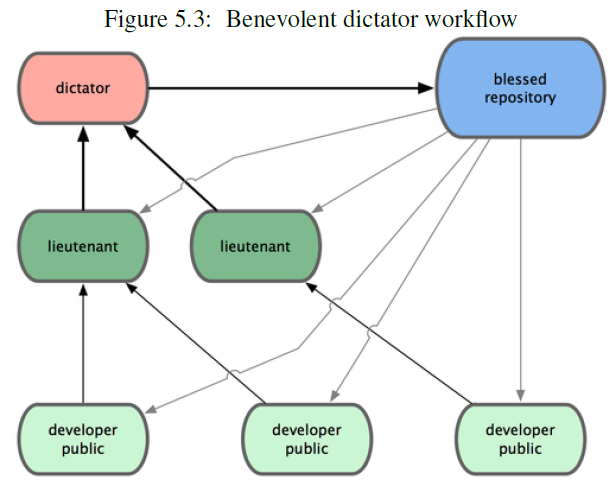
\includegraphics[scale=0.85]{figures/federatedGit.png}
	\caption[A distributed workflow to control for volatile versioning behavior.]{A distributed workflow to control for volatile versioning behavior.  From  \cite{cederqvist2002version}.}
	\label{fig:federated}
\end{figure}

\section{Structured Data}

The \gls{rdfa} framework encodes \gls{linked} vocabularies into \gls{html} documents, and provides an opportunity to make change logs machine interpretable. \cite{Adida2015}.
\begin{figure}
	\centering
	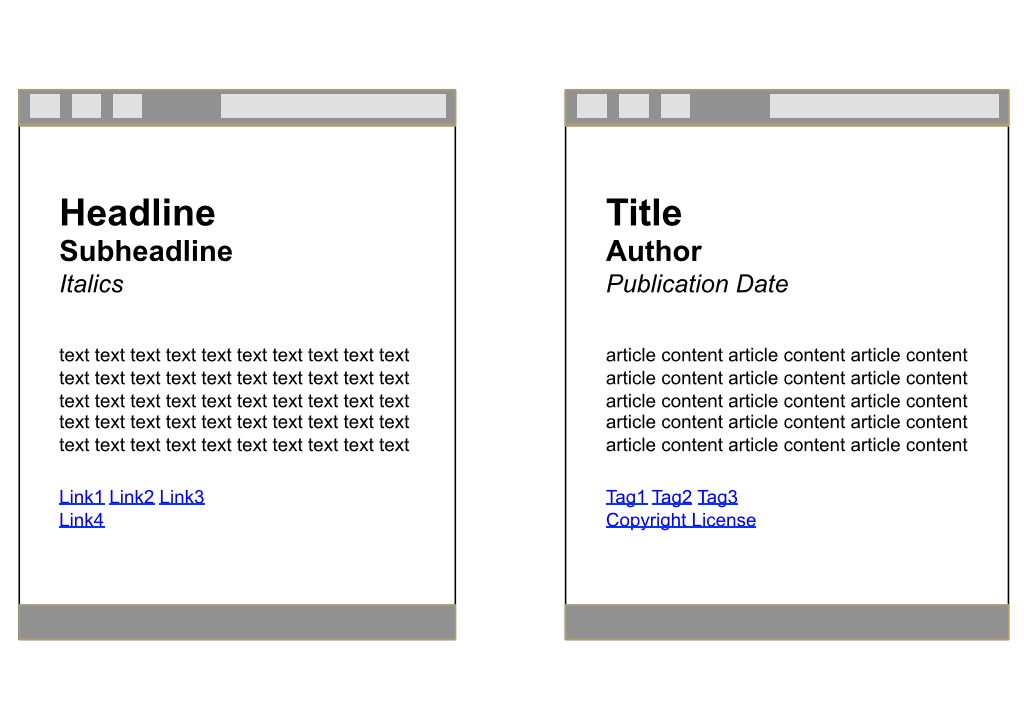
\includegraphics[scale=0.40]{figures/RDFaSemantics.png}
	\caption[Illustration of the difference in what autonomous systems see when crawling a web page and what humans see when reading the same material.]{Illustration of the difference in what autonomous systems see when crawling a web page and what humans see when reading the same material. Figure 1 from \cite{Herman2015}}
	\label{RDFa}
\end{figure}Figure \ref{RDFa} illustrates the semantic difference between what web crawlers and what humans see when they consume web pages.
People intuitively understand that certain strings represent meaningful information based on location and style.
\gls{rdfa} seeks to encode that understanding natively for effective machine consumption.
Extending this approach into publishing change logs, will allow linked data to capture the metaphorical meat of change content.

The implementation requires changing publishing practices from plain-text documents to something structured-data compatible such as \gls{html}.
The change also has the added benefit of making the logs available on-line, and thus, more openly accessible to data users through the utilization of web based search engines.
Large companies such as Google have already begun equipping their web crawlers to consume structured data such as \gls{rdfa} from web pages.
\gls{rdfa} has already had significant success in adoption across a variety of web publication platforms and eases the search for their content \cite{Bizer2013}.
The design of \gls{rdfa} focuses on describing the web page's content through markup \cite{Herman2015}.
The underlying or resulting versioning data model may not conform with the format of content presented in the change log.
Poor affinity would lead to a poorly structured graph or missing content, undermining the value gained by encoding linked data into the change log.
As a result, another method using \gls{jsonld} was pursued since its purpose is to store data separate from visible content.

The \gls{json} data format allows web pages to store data for JavaScript applications within the document.
It utilizes a simple and robust syntax to accommodate a wide variety of content.
\gls{jsonld} extends the original specification by defining rules which allow entries to resolve as web vocabularies, giving them a meaningful context \cite{JSONLD}.
Because it stores data separate from visible content, \gls{jsonld} does not need to adhere with the constraints of visible content.
Every linked data triple must instead be explicitly defined, meaning that resulting documents may likely be much larger than their \gls{rdfa} counterparts.

\section{Change Distance}

A major function of versions is to communicate the amount of change which exists between two versions.
The quantity plays a major role in determining the freshness of data within a collection, indicating its pertinence to new projects \cite{Bouzeghoub:2004:FAD:1012453.1012464}.
Additionally, changing versions are often used to signal other applications downstream that a new version may be necessary to adopt data improvements \cite{TILMES2011548}.
Many efforts currently to compute a distance measure relies on data provenance.
Formalizing operations on provenance remains an active field of research \cite{Ainy:2015:ASD:2806416.2806429}.
Other approaches relate to determining semantic similarity in trying to summarize the data set and computing a distance measure \cite{Hliaoutakis06informationretrieval}.

\subsection{Provenance Distance}

Previous endeavors to extract insight into data set performance or behavior using provenance have provided exciting results \cite{dai2014provenance}.
The research, however, generally studies the current state of an object's provenance rather than compare two provenance graphs.
As stated previously, versions result from slight variations between the provenance of two objects.
The connection suggests that studying the variations' magnitudes will help predict the change's impact.
The measurement known as \gls{provdist} seeks to determine the impact of changes in provenance on new data versions through measuring graph edit distances.

\begin{figure}
	\centering
	\begin{adjustbox}{addcode={\begin{minipage}{\width}}{
					\caption[Provenance graph of a Level 3 data product, showing the inter-relations between different data products in generating the final product.]{Provenance graph of a Level 3 data product, showing the inter-relations between different data products in generating the final product.  Figure 2 from \cite{TILMES2011548}\label{ProvGraph}}\end{minipage}},rotate=90,center}
		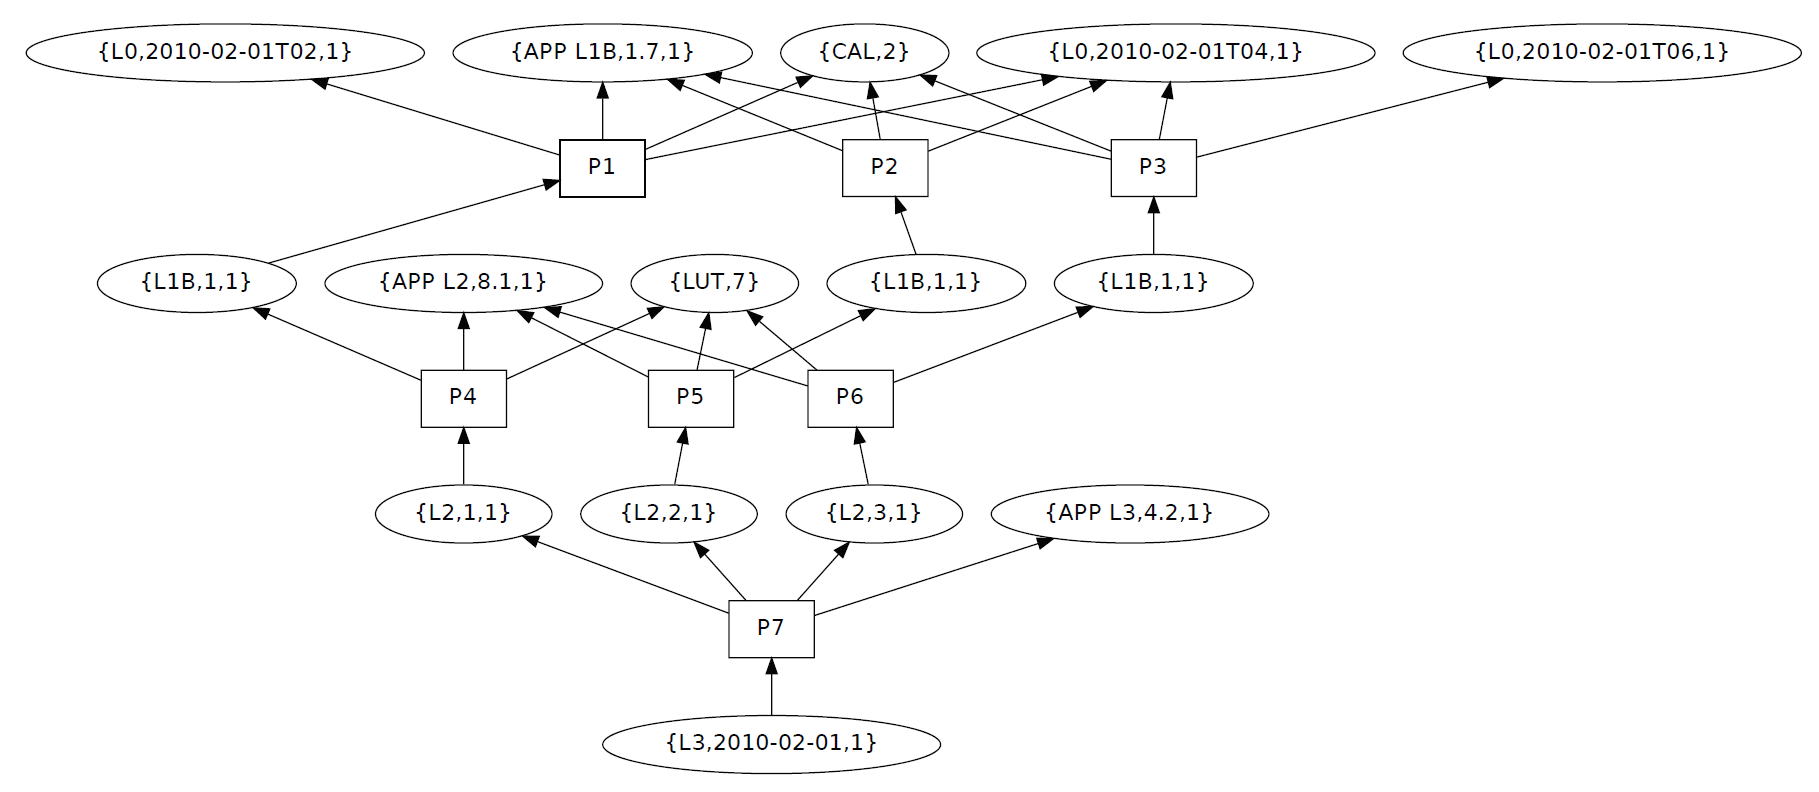
\includegraphics[scale=0.45]{figures/OzoneProvGraph.png}
	\end{adjustbox}
	
\end{figure}

The first ingredient necessary to calculate provenance distance is a linked data graph capturing the sequence of events leading to the old and new objects' creation, like the one shown in Figure \ref{ProvGraph}.
The graph shows the multiple lower level products involved in creating a Level 3 ozone indicator.
This can be accomplished through the use of previously mentioned provenance models, but these graphs are not widely available.
Using PROV to represent provenance data in a semantic model produces an acyclic directed graph with labeled nodes.
As a result, the provenance distance problem reduces to similarity measurement.
When calculating the similarity measurement of two graphs, algorithms determine how far the graphs are from being isomorphic \cite{Cao2013}.
Node labeling simplifies the similarity measurement process by providing nodes which must match together, and greatly reduces the complexity from computing generalized graphs.
Graph Edit Distance, counting the edits necessary to transform one graph into another, provides a quantitative measure to associate with this process  \cite{Gao2010}.
Some variations count edge changes \cite{Goddard:1996:DGU:246962.246972}.

In Figure \ref{GraphEdit}, the left graph transforms through a move of edge 1 and a rotation of edge 4, resulting in an edit distance of two.
Such changes in a provenance graph would demonstrate an alteration in dependencies between objects used to generate a final notable product.
Isolating changes responsible for differences in provenance can become difficult in complex environments as Tilmes observes in 2011, 
\begin{quotation}
	Consider the relatively common case of the calibration table, which is an input to the L1B process, changing. Even though the version of the L2 or L3 software hasn't changed, the data files in the whole process have been affected by the change in the calibration.
\end{quotation} \cite{TILMES2011548}.
L-number is shorthand for the level system featured in Figure \ref{NASALevels}.
While provenance distance may be straight-forward to calculate, the indicator hides many insights into an object's behavior.

\begin{figure}
	\centering
	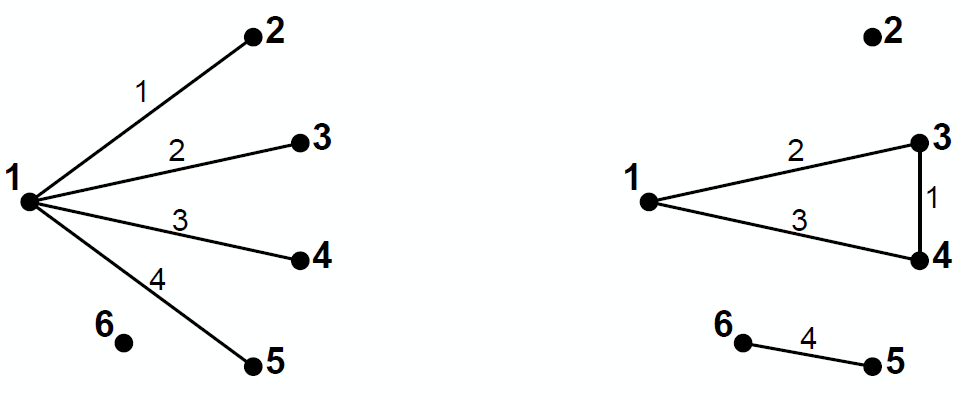
\includegraphics[scale=0.40]{figures/GraphEdit.png}
	\caption[The labeled graph on the left transforms into the right graph under two edge edits.]{The labeled graph on the left transforms into the right graph under two edge edits. Figure 2 from \cite{Goddard:1996:DGU:246962.246972}}
	\label{GraphEdit}
\end{figure}

Methods to provide quality of service boundaries leveraging provenance already exist which compare workflows based on performance criteria \cite{2015:CAA:2778374.2778504}.
These procedures focus primarily on quick retrieval and efficient storage instead of capitalizing on the latent information accessed by reasoning across data set versions \cite{tan2004research}.
Using only provenance data is insufficient to give insight into a change's impact because it does not provide information on structural or content differences which is what change logs provide.
Measuring a change's impact with accuracy comparable to a change log requires a more detailed understanding and description than provenance can provide  \cite{Bose:2005:LRS:1057977.1057978}.
Sufficiently precise versioning measurements cannot be provided by provenance distance, but it could indicate the confidence of versioning results, which is out of scope for this project.

\section{Summary}

In order to better formalize data versioning information, an approach must be developed leveraging common aspects of very disparate versioning systems.
A data model based around versioning operations instead of impact remains largely untouched across the field.
Version identifiers must additionally be untangled from communicating change distance which change logs accomplish with greater detail.
The logs, in turn, need to be extended for machines to consume, easing adoption as data set size grows through automation.
Change measures utilizing version graphs rather than provenance graphs are also under-explored.
Chapter \ref{ch:model} presents a model to create a versioning graph.

%%% Local Variables:
%%% mode: latex
%%% TeX-master: t
%%% End:
